\documentclass[12pt,a4paper]{article}
\usepackage[a4paper, total={6in, 9.5in}, headsep=0.5in]{geometry}
\usepackage[utf8]{inputenc}
\usepackage[T1]{fontenc}
\usepackage{ebgaramond}
\usepackage{amssymb,amsmath,amsfonts}
\usepackage{fancyhdr}
\usepackage{array}
\usepackage[nottoc]{tocbibind}
\usepackage{biblatex}
\usepackage{color}
\usepackage[urlcolor=blue]{hyperref}
\hypersetup{colorlinks=true, linktoc=all, linkcolor=black}
\usepackage{enumitem}
\usepackage{setspace}
\usepackage{xcolor}
\usepackage{listings}
\usepackage{multicol}
\usepackage{wrapfig}
\usepackage{graphicx}
\usepackage{titlesec}
\usepackage{lmodern}
\usepackage{lipsum}
\usepackage{cfg/psl-cover}
\addbibresource{bibliographie.bib}

\titleformat{\subsection}[block]
  {\normalfont\large\bfseries}   
  {\thesubsection}               
  {1em}                          
  {}                             

\titlespacing*{\subsection}{0.5cm}{10pt}{5pt}

\titleformat{\subsubsection}[block]
  {\normalfont\large\bfseries}   
  {\thesubsubsection}               
  {1em}                          
  {}                             

\titlespacing*{\subsubsection}{1cm}{10pt}{5pt}

\lstset{language=C, keywordstyle={\bfseries \color{blue}}}
\onehalfspacing

\title{CSI Première année}
\author{Salomé Gobbi}
\date{May 2025}


\pslassetspath{pls-assets}

\newcommand{\todo}[1]{{\color{red}\textbf{TODO} \textit{#1}}}


\title{
Interface de création basée sur l'IA pour la stimulation de l'incarnation d'un acteur
\\
\vspace{1cm}
AI-based creative interface for enhancing the embodiment of an actor
}

\author{Salomé Gobbi}

\institute{Mines Paris - PSL}
\doctoralschool{ISMME}{621}
\specialty{Informatique temps réel, robotique et automatique}
\date{27 Juin 2025}

\jurymember{1}{Daniel Pressnitzer}{}{}
\jurymember{2}{Brian Ravenet}{}{}


\begin{document}
\maketitle{}

\renewcommand{\contentsname}{Sommaire}
\tableofcontents
\newpage

\pagestyle{fancy}
\renewcommand\headrulewidth{1pt}
\fancyhead[L]{
\includegraphics[scale=1.3]{MinesParis-PSL-CtreDeRobotique2_logo-300x89.jpg}}
\fancyhead[C]{\small{CSI Première année - Salomé Gobbi \\ \textsc{}}}
\fancyhead[R]{}

\newpage
\input{Introduction}

\newpage
\section{Répétition Theatrale}

Afin de comprendre les enjeux de notre projet, nous avons commencé par étudier les différentes techniques de répétitions utilisées dans un contexte de quete de sens du texte et d'ancrage dans le personnage a incarner. 



\subsection{Recherche Interieure: Le systeme de Stanislavski et la Méthode} 
Stanislavski fait partie d'un des premiers theoriciens de la répétition théatrale,  


\subsection{Recherche Exterieure: Travail du corps}



\newpage
\input{RepetitionVR/RepetitionEnVR}

\newpage
\section{Etude pilote}

Le but a terme étant de créer une plateforme de répétition en réalité virtuelle intégrant des outils d'IA, nous avons décidé dans un premier temps d'aller sonder les utilisateurs de cet outil, les comédiens, dans une étude pilote ayant pour but d'identifier leurs besoins spécifiques. 

\subsection{Objectif de l'étude}
Lors de cette première étude pilote en présence de comédiens, 
nous avons décidé de se pencher sur le travail d'un monologue en
réalité virtuelle et en particulier sur l'effet de l'environnement 
sur ce travail de monologue. 

Le but de l'étude de ce travail, lors duquel le comédien s'approprie le texte et se plonge dans 
le personnage, est de répondre à plusieurs questions de recherche qui sont les suivantes: 

\begin{itemize}
    \item L'utilisation de l'outil qu'est la réalité virtuelle affecte-t-elle la présence ressentie des comédiens dans leurs roles? Et si oui, comment?
    \item Est-ce que le fait de pouvoir moduler son environnement d'immersion affecte la présence ressentie des comédiens dans leurs roles? Et si oui, quels éléments de l'environnement jouent le plus grand role?
    \item Est ce que le niveau de liberté dans la modulation de cet environnement va avoir un impact sur l'acceptation de ce dernier et sur son influence sur les comédiens? 
\end{itemize}

En partant d'un choix de monologue, le tableau VI de Roberto Zucco de Bernard-Marie
Koltes, nous avons dans un premier temps tiré trois types d'environnements d'immersion 
de nature esthétiques différentes qui permettent d'évaluer quels types de significations 
d'objets vont avoir de l'importance. Les 3 natures esthetiques sont: 
\begin{itemize}
    \item Environnement scénographique: un environnement qui suit les didascalies et qui représente le lieu qui serait représenté sur un plateau
    \item Environnement narratif: un environnement qui illustre les paroles du personnage afin d'immerger le comédien dans son propre récit
    \item Environnement abstrait/émotif: un environnement qui a pour but de susciter chez l'acteur l'état affectif que provoque le sens du texte et son thème 
\end{itemize}

Lors de cette étude, le comédien va pouvoir être en immersion dans 3 environnements différents qui ont été imaginés pour rentrer
dans chacune des ces trois catégories esthétiques. Dans cette scène, Le personnage principal éponyme revendique son invisibilité 
sociale et son conformisme discret, affirmant ne pas être un héros, mais un être ordinaire qui suit sans dévier le cours d'une vie
silencieuse et sans éclat dans l'épais brouillard de la vie. Dans ce contexte la, nous avons modélisé pour la première catégorie, une 
station de métro puisque c'est dans une station de métro que se passe cette scène. Pour la deuxième catégorie, nous avons modélisé un
amphithéatre d'université puisque son monologue évoque sa place dans les rangs des élèves de la Sorbonne. Finalement, pour la troisième 
catégorie, nous avons modélisé un épais brouillard avec une foule de personnages s'affairant autour du comédien pour évoqué le sentiment d'invisibilité dans l'épais brouillard de la vie ordinaire.
Dans ces trois cas, le comédien va soit se voir l'environnement entièrement imposé, soit il aura la possibilité de moduler certains aspects
de celui-ci avec un menu déroulant. En fonction de l'environnement dans lequel il se trouve, l'acteur pourra modifier la taille de la pièce, la luminosité, et
y ajouter et déplacer des objets afin de créer l'espace autour de lui de sorte à ce qu'il fasse écho au sens peronnel du texte qu'il s'approprie. 

\begin{figure}[h]
  \centering

  \begin{minipage}[b]{0.31\textwidth}
    \centering
    \includegraphics[width=\textwidth]{images/metro1.png}
  \end{minipage}
  \hfill
  \begin{minipage}[b]{0.33\textwidth}
    \centering
    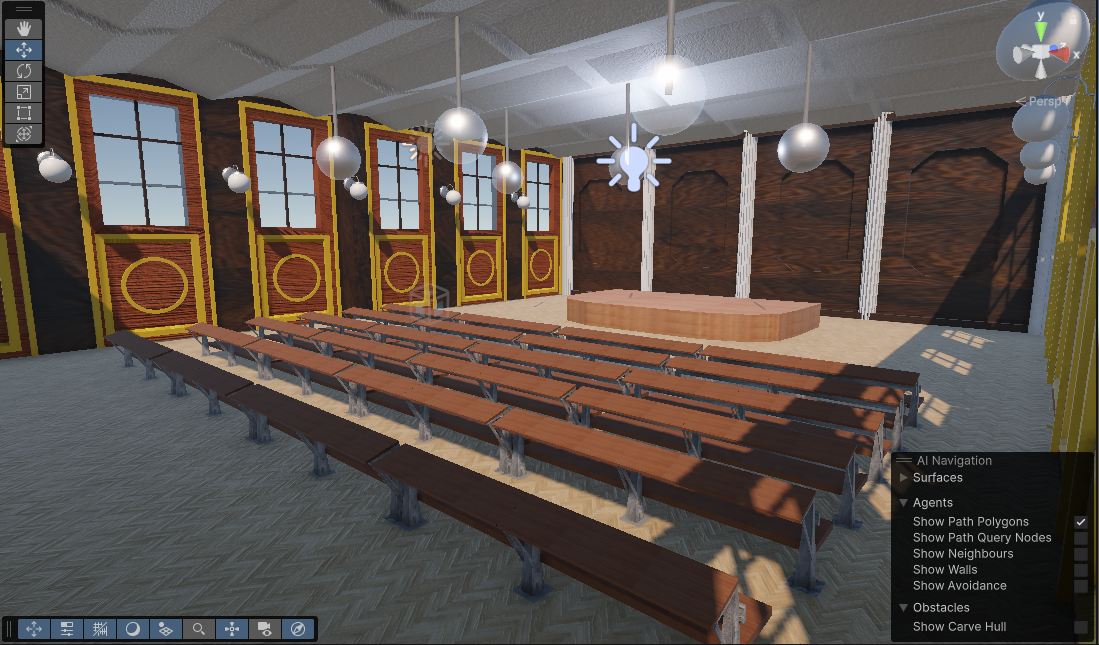
\includegraphics[width=\textwidth]{images/Amphi.png}
  \end{minipage}
  \hfill
  \begin{minipage}[b]{0.32\textwidth}
    \centering
    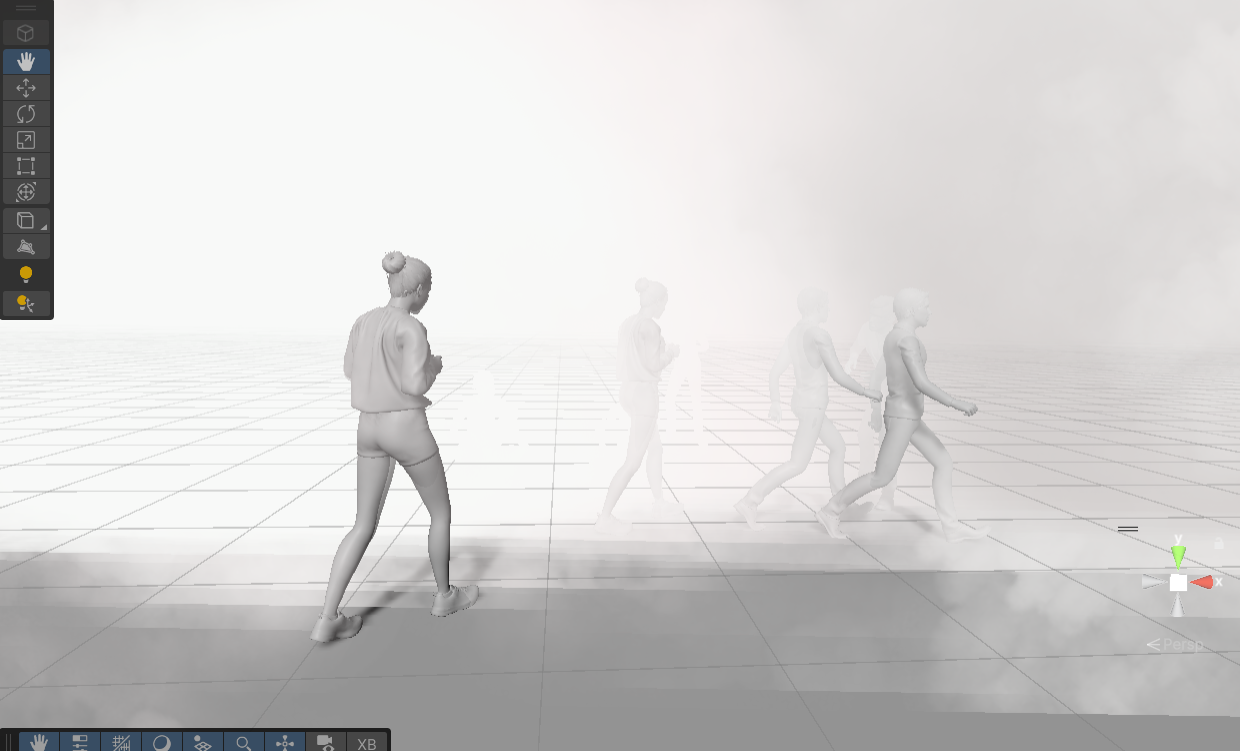
\includegraphics[width=\textwidth]{images/Fog3.png}
  \end{minipage}

  \caption{Captures d'écran des 3 environnements (de gauche à droite: scénographique, narratif, abstrait)}
  \label{fig:trois_images}
\end{figure}

\subsection{Protocole}



\subsection{Conclusions}








\newpage
\section{Intégration de l'IA}
À la suite de l’analyse des résultats et des retours issus de notre étude pilote, une prochaine étape 
essentielle consiste à intégrer des outils d’intelligence artificielle au sein de notre environnement
de répétition théâtrale en réalité virtuelle, et à interroger leur pertinence dans ce contexte spécifique.
L’IA offre en effet la possibilité de générer dynamiquement des décors virtuels en fonction du texte, 
de l’émotion recherchée ou de l’univers esthétique souhaité par le metteur en scène, et de les faire 
évoluer en temps réel selon les besoins du travail scénique. La nature des éléments générés, tout comme
les modalités d’interaction entre l’utilisateur et l’IA au cours des différentes étapes du processus de 
création, peuvent varier considérablement. Cette section se propose d’explorer ces possibilités et d’en 
analyser les enjeux.

\subsection{Nature des objets générés}
\subsubsection{Génération d'images et de vidéos 360 degrés}
\paragraph{}
Dans certaines applications de réalité virtuelle, l'utilisation d'images et de vidéos panoramiques
 à 360° peut s’avérer pertinente. En effet, pour certains types d’environnements, une image statique 
 peut suffire à transmettre une ambiance ou une intention visuelle, sans nécessiter la construction 
 complète d’un espace 3D, souvent plus coûteux en termes de génération et de calcul. Ces dernières 
 années, la génération d’images de haute qualité a connu des avancées significatives 
 \cite{li2025comprehensive}, avec l’essor des modèles de diffusion qui tendent à supplanter les GANs (generative
 adversial networks). Dans un contexte immersif, la génération d’images par IA peut être 
 exploitée de différentes manières :

\begin{itemize}
\item \textbf{Création d’éléments 2D intégrés à la scène} : tels que des tableaux, écrans d’affichage, 
panneaux de signalisation ou affiches. Ces éléments peuvent enrichir visuellement l’environnement sans 
recourir à des objets 3D complexes.

\item \textbf{Génération de textures et de matériaux} : la création dynamique de textures permet de
modifier l’apparence d’un environnement (éclairage, température de couleur, ambiance générale) sans
altérer sa géométrie \cite{CHEN2024112113}.

\item \textbf{Création de décors de fond panoramiques} : la génération d’images 360° (skyboxes) à partir
 de descriptions textuelles \cite{chen2023text2lightzeroshottextdrivenhdr} permet de simuler des 
 paysages lointains ou des environnements secondaires. Bien que ces décors soient moins immersifs que 
 des scènes entièrement modélisées en 3D, ils restent efficaces pour compléter un espace visuel. Par 
 exemple, dans l’une des scènes de notre étude pilote, des skyboxes générées à l’aide de SkyboxAI 
 représentaient l’extérieur visible à travers les fenêtres d’un amphithéâtre virtuel.

\end{itemize}

\subsubsection{Génération d'objets}
\paragraph{}
La génération d'objets 3D est une des utilisations les plus répandues de l'IA générative pour utilisation
en réalité virtuelle, que ce soit pour les développeurs mais aussi pour les utilisateurs. 
Afin de peupler un environnement existent, l'utilisateur pourrait avoir recours a de la génération d'objets 3D. 
En prenant l'exemple de notre étude pilote, le comédien pourrait avoir l'opportunité de prompter une IA pour
rajouter des éléments qui ne seraient pas présents dans le catalogue proposé. Il existe plusieurs natures d'objets 
3D et plusieurs facons de les générer:

\begin{itemize}
    \item Recherche d'objets présents dans une base de données existente: un des enjeux majeurs de la VR 
    reste la rapidité et l'économie de la puissance de calcul. Il est donc possible de réduire le temps de génération
    ainsi que la puissance de calcul nécéssaire grace a des algorithmes qui vont comprendre la requete de l'utilisateur
    et la comparer aux objets deja modélisés. C'est ce qu'entreprend un des blocs de l'architecture du LLMR, Large Language Model for Mixed 
    Reality (\cite{delatorre2023llmr}), en allant chercher dans la base de donnée SketchFab pour voir s'il existe un 
    modèle existent de l'objet demandé. 
    \item Génération d'objets Text to 3D: cette technique englobe tous les processus différents qui permettent 
    la génération automatiques d'objets 3D a partir d'une description textuelle. Bien qu'il existe un grand nombre
    de techniques différentes, le pipeline classique commence par l'interprétation sémantique du texte, suivie de la 
    synthèse d'une représentation volumétrique intermediaire (nuages de points, champ de densité implicite, image de profondeur), 
    avant d'etre converti vers un maillage 3D permettant le rendering. Parmis les techniques les plus récentes, il y a DreamFusion
    (\cite{poole2022dreamfusion}), qui utilise un modèle de diffusion text to image deja entrainé afin d'optimiser des modèles 3D initialisés aléatoirement (sous forme de Neural Radiance Fields) sans
    avoir recours a une base de données annotée de données 3D. OpenAI aussi travaille sur un modèle appelé Shap-E (\cite{jun2023shap}), qui génère des représentations
    implicites qui peuvent ensuite etre convertie en mesh ou en neural radiance field. 
    \item Génération d'objets animés et interactifs
\end{itemize}

dans l'etude pilote, les comédiens ont vocalisé l'envie/besoin d'avoir des objets 
animés/interactifs 
\subsubsection{Génération d'environnements 3D}
\paragraph{}
On peut aussi générer des environnements entiers 



\subsection{Nature de l'intervention (facon de communiquer avec l'IA)}
\subsubsection{Aucune intervention de l'utilisateur}
\subsubsection{Prompting textuel}
\subsubsection{Prompting vocal}
\subsubsection{Prompting gestuel}
\subsection{Niveau de l'intervention (personnalité de l'IA)}
\subsubsection{Prompted or independent AI}
\subsubsection{Incremental or instantaneous AI}
\subsubsection{Pleasing or provoking AI}

\newpage
\section{Bibliographie}
\printbibliography

\end{document}
 